% Drawing 154/07-22 -- folder 154, batch 07, archive page 132 (PDF page 133).
% Transcription: au-dessous, un croquis au crayon : un cercle partagé en secteurs marqués $D_1, \ldots, D_8$, un axe fléché passant par le centre
% Kind: octagon of sectors D1..D8 with an arrowed axis. Method 2 (schematic redraw from the facsimile). Status: partial.
% Notes: A faint pencil circle and inside it an octagon drawn in heavier strokes, four lines through its centre cutting it into eight sectors, the letters D_1 to D_8 written outside the sides, counter-clockwise from the upper right; a thick axis through the centre with an arrowhead at each end and a small cross-stroke near each end; a marked point on the axis in the lower left and a light green blot on it in the upper right. The indices are small on the page: D_1, D_2, D_5, D_6, D_7 are read, the others are placed by the order (the one on the right could be read D_3 as well as D_8). Redrawn 2026-11-12 (issue 128): to check again.
% Coordinates: 1 unit = 1 mm = 1/100 of the crop width (bbox in page fractions: [0.58, 0.395, 0.695, 0.485]).
% Redrawn by Claude (claude-fable-5-2), issue #128, 2026-11-12; not checked by a human; not compiled (no TeX in the session).
% Rights: reproduces part of the work -- behind RENDER_TRANSCRIPTS, never published by itself.
\documentclass[tikz,border=3pt]{standalone}
\usepackage{amsmath,amssymb}
\usetikzlibrary{patterns,arrows.meta}
\tikzset{pencil/.style={black!45}, struck/.style={black!35}, mpt/.style={circle,draw,inner sep=1.3pt}, pt/.style={circle,fill,inner sep=0.9pt}, opt/.style={circle,draw,fill=white,inner sep=1.1pt}}
\begin{document}
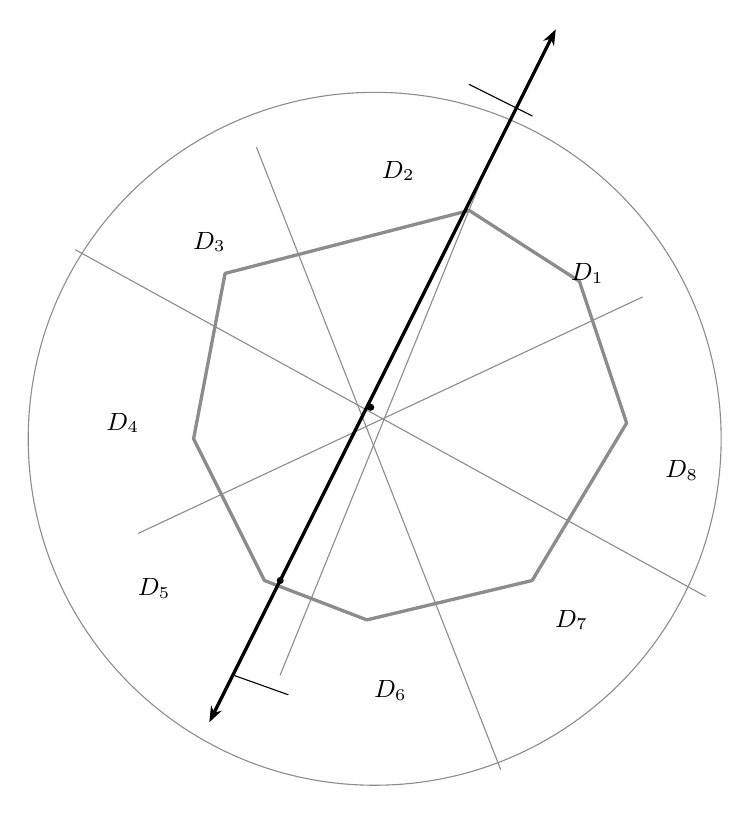
\begin{tikzpicture}[x=1mm,y=1mm,line cap=round,line join=round,font=\scriptsize]
\draw[pencil] (48,-62) circle[radius=44];
\draw[pencil,very thick] (60,-33) -- (74,-42) -- (80,-60) -- (68,-80) -- (47,-85) -- (34,-80) -- (25,-62) -- (29,-41) -- cycle;
\draw[pencil] (10,-38) -- (90,-82);
\draw[pencil] (33,-25) -- (64,-104);
\draw[pencil] (18,-74) -- (82,-44);
\draw[pencil] (62,-28) -- (36,-92);
\draw[very thick,{Stealth[length=2mm]}-{Stealth[length=2mm]}] (27,-98) -- (71,-10);
\draw (60,-17) -- (68,-21);
\draw (30,-92) -- (37,-94.5);
\node[pt] at (47.5,-58) {};
\node[pt] at (36,-80) {};
\node[inner sep=1pt] at (75,-41) {\small $D_1$};
\node[inner sep=1pt] at (51,-28) {\small $D_2$};
\node[inner sep=1pt] at (27,-37) {\small $D_3$};
\node[inner sep=1pt] at (16,-60) {\small $D_4$};
\node[inner sep=1pt] at (20,-81) {\small $D_5$};
\node[inner sep=1pt] at (50,-94) {\small $D_6$};
\node[inner sep=1pt] at (73,-85) {\small $D_7$};
\node[inner sep=1pt] at (87,-66) {\small $D_8$};
\end{tikzpicture}
\end{document}
